% ---------------------------------------------------------------
% Sections 2 and 3. Elective surgical capacity in Goi\'as, 2019-2025.
%
% All TODO/VERIFY markers resolved; none remain in this file.
% ---------------------------------------------------------------

\section{Setting and data}
\label{sec:data}

\subsection{Institutional background}

Brazil's Sistema Unico de Sa\'ude (SUS) provides universal hospital care free at
the point of use. Access to elective surgery is rationed by queue rather than by
price, and queue length is the operative constraint on what patients receive:
patients enter a queue managed by state or municipal
regulatory authorities, wait, and are then assigned to a facility that may or
may not be in their municipality of residence. The assignment is made by an
administrative regulation system rather than by patient choice, which makes the
allocation rule an object of policy and, in principle, an object of design.

We study the state of Goi\'as, in Brazil's Centre-West region, over the period
January 2019 to December 2025. Three policy events bracket the period. First,
the state health secretariat (SES-GO) restructured its surgical regulation
during 2021 and 2022, including the transfer of a number of municipal hospitals
to state management and the introduction of a consolidated queue.
The restructuring is not dated from its instruments; the break dates in Section~\ref{sec:breaks} are estimated from the admission series alone and are not attributed to it. One instrument has been read: Resolu\c{c}\~ao CIB
n.\ 111/2021 of 15 July 2021, which approves the state protocol for the regulation of elective surgery. It makes the
SWALIS priority classification form mandatory for elective surgery requests, routes requests through the state elective
surgery regulation system (REGNET), and orders that patients be sequenced and ties broken automatically with weights, SWALIS
priority carrying the greatest weight and ties broken by the longer wait. We do not claim that it caused any change in the data
below; SIH records no queue entry date and therefore no waiting time. Second, the federal government established the Programa
Nacional de Redu\c{c}\~ao de Filas (PNRF) by Portaria GM/MS n.\ 90 of 3 February
2023. Third, the federal Programa Mais Acesso a Especialistas (PMAE) began
disbursing in 2025; we use its start only to date the final regime boundary and
make no claim about its allocation across states.

\subsection{Data}

What the data cover. SIH/SUS records SUS-financed hospital authorisations (AIH) processed by facilities in the
state, so it is not the full inpatient record: care paid for privately or through health plans is absent. Residents of
Goi\'as treated in another state appear in that state's files. In Distrito Federal (official DATASUS files RDDF), Goi\'as
residents account for 3{,}481, 3{,}005 and 3{,}995 elective surgical AIH in 2019, 2023 and 2025, which is 7.0, 3.7
and 4.0 per cent of the elective surgical admissions of all Goi\'as residents, and 25 to 51 per cent for the three Entorno
municipalities named in Section~\ref{sec:flows}. The model's demand therefore omits those admissions. Records of residents
of other states treated in Goi\'as (0.7, 0.2 and 0.3 per cent of elective surgical AIH) are dropped by the in-state filter.

Our source is the Sistema de Informa\c{c}\~oes Hospitalares do SUS (SIH/SUS), the
national hospital billing system. Each record is an \emph{Autoriza\c{c}\~ao de
Internacao Hospitalar} (AIH), the authorisation document that accompanies an
admission and against which the facility is reimbursed. We use the reduced
(RD) files for Goi\'as for all 84 months from January 2019 to December 2025,
retrieved from the DATASUS public FTP server and converted from the proprietary
DBC format to Parquet. The ingestion is scripted and accompanied by a
reproducibility manifest recording file hashes and retrieval dates.

The full extract contains 2{,}719{,}254 AIH records. We restrict attention to
surgical admissions, defined as records whose procedure code (\texttt{PROC\_REA})
falls in group 04 of the SIGTAP procedure table, and within those we
distinguish elective admissions (\texttt{CAR\_INT} $=$ 01) from urgent
admissions (\texttt{CAR\_INT} $=$ 02). This yields 430{,}802 elective surgical
admissions across 201 distinct facilities identified by their CNES
establishment code. Group 04 is the surgical block of the SIGTAP table and includes obstetric
surgery: scheduled caesarean sections account for 2{,}431 elective admissions in
2023, roughly 3 per cent of the year's volume. We retain them, since a scheduled
caesarean consumes operating-room and surgical bed capacity on the same terms as
any other elective procedure, and the bed-day denominator in
Section~\ref{sec:results} includes obstetric-surgical beds correspondingly.

Three variables carry most of the analysis. \texttt{COMPETENCIA} is the
processing month, that is, the month in which the AIH was submitted for
payment. \texttt{DT\_INTER} is the admission date. \texttt{GESTAO} records
whether the admission was billed under state or municipal management.
We use it only to
label admissions in Figure~\ref{fig:scatter}; the provider grouping that carries
the analysis in Section~\ref{sec:results} is taken from the CNES field
\texttt{TP\_GESTAO}, which records contract-administration authority at facility
level and is independent of the SIH billing code.


\begin{table}[t]
\centering
\caption{Flow of hospital authorisations (AIH) into the analysis sample, SIH/SUS RD files processed in Goi\'as (RECORD-style).}
\label{tab:recordflow}
\begin{tabular}{lrrr}
\toprule
 & 2019 & 2023 & 2025 \\
\midrule
All AIH processed in Goi\'as & 350{,}564 & 423{,}932 & 467{,}575 \\
Surgical procedures (group 04) & 150{,}243 & 192{,}504 & 214{,}762 \\
Elective (CAR\_INT 01) & 46{,}748 & 79{,}440 & 96{,}154 \\
Resident in a Goi\'as municipality (IBGE list) & 46{,}414 & 79{,}247 & 95{,}848 \\
At the model's facilities (net bed budget $> 0$) & 46{,}391 & 74{,}832 & 87{,}506 \\
Facilities in the model & 131 & 131 & 145 \\
\bottomrule
\end{tabular}
\end{table}

\subsection{Two measurement concerns}
\label{sec:measconc}

\paragraph{Processing month versus admission month.}
SIH records are indexed by processing month, not by the month in which the
surgery took place. If submission practice changed, a change in the indexed
series would not correspond to any change in surgical activity. The median
submission lag over our period is zero months and the mean is 0.70 months, but
it is not constant: the mean lag for elective admissions rises from 0.42 months
in calendar 2021 to 0.65 in calendar 2022, while the lag for urgent admissions is flat at 0.82 to
0.87 throughout. We therefore reconstruct every series on \texttt{DT\_INTER}
and report both. The reconstruction is reported in Table~\ref{tab:falsification}
and does not change any conclusion. Series indexed on admission date are
right-censored at the end of the panel, because admissions late in 2025 are
still being processed; we truncate them accordingly.

\paragraph{Reporting reliability.}
Facility-level reporting in SIH is uneven. Of the 201 facilities in the
extract, the median has non-missing data in 95.2 per cent of the months within
its own reporting span, but the tenth percentile has only 51.2 per cent. Some
facilities bill in batches: one unit records 1{,}171 elective cases in May 2022
and zero in thirteen other months of 2022 and 2023. Facility-level statistics
computed naively on this panel are unreliable, since a facility that suspends
and resumes reporting is indistinguishable from one that suspends and resumes
operating.

We therefore define a \emph{reliable subset}: facilities reporting in at least
95 per cent of the months within a span of at least 60 months, with at least
500 elective surgical cases over the panel. Sixty-one of 201 facilities meet
this definition, and they account for 76.2 per cent of all elective surgical
volume.

A second rule applies wherever a facility-level growth ratio is computed. A
facility averaging under five elective cases per month in the base window of a
ratio is excluded from that ratio, because a denominator of one or two cases
produces a quotient that is noise rather than growth. The rule is applied to the
base window of each comparison separately, so the subset it leaves differs by
comparison and is named at each use. It is not doing the work: recomputing both
facility-level findings on all 61 leaves them intact, as reported below. Aggregate series are reported for the full sample; all facility-level
results, and all break tests intended to be conclusive, are reported for the
reliable subset.

% ---------------------------------------------------------------

\section{Results}
\label{sec:results}

\subsection{A structural change in elective surgical volume}
\label{sec:breaks}

Figure~\ref{fig:ratio} plots the monthly ratio of elective to urgent surgical
admissions in Goi\'as from 2019 to 2025. We use the ratio rather than the level
of elective admissions. Urgent surgical volume provides a descriptive comparison series because it is recorded through the same administrative system. Emergency surgical demand is not scheduled, is not subject to
administrative queue management, and flows through the same facilities, the
same billing pipeline and the same authorisation process as elective surgery.
Over the seven-year panel it stays between roughly 7{,}000 and 10{,}500
admissions per month with no discontinuity. It is not a control group: changes in demand, coding or reporting need not affect urgent and elective admissions equally.

The series has a clear validity check built into it. In April 2020, when
Brazilian states suspended elective procedures in response to COVID-19, the
ratio falls to 0.196 from a 2019 average of 0.452. The measure detects a known
suspension of elective activity at the correct month and with the correct sign.

\begin{figure}[t]
\centering
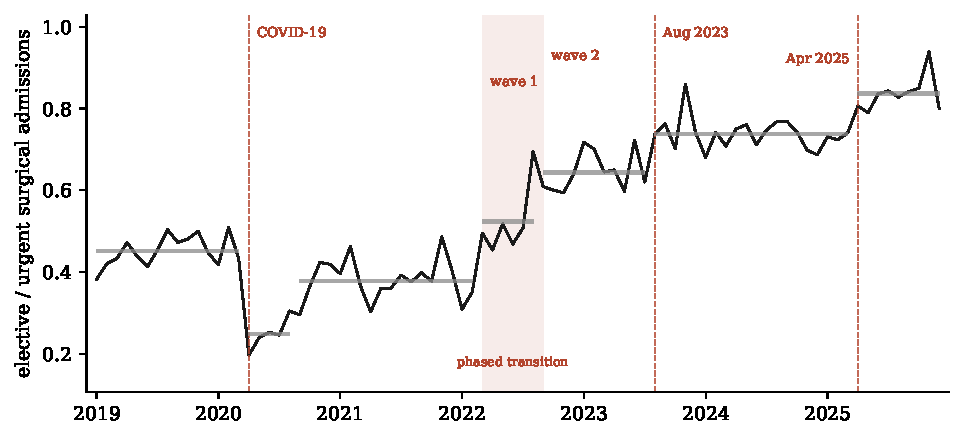
\includegraphics[width=\textwidth]{fig1_ratio_series.pdf}
\caption{Monthly elective-to-urgent surgical admission ratio, Goi\'as, 2019-2025.
Grey horizontal segments are within-regime means. Dashed vertical lines mark
the regime boundaries discussed in the text. The COVID-19 boundary at April
2020 is recovered by the changepoint procedure without being imposed.}
\label{fig:ratio}
\end{figure}

We locate regime changes using the PELT changepoint algorithm
\citep{killick2012} with an RBF cost, applied to the ratio series. To avoid
selecting break dates that we had already formed views about, we report the
procedure's output across penalty values rather than a single specification,
and we cross-check against a fixed-cardinality dynamic-programming search.
The procedure returns locations but not confidence intervals; see
Section~\ref{sec:limits}.

The procedure returns five boundaries at penalty 1.0 on the full sample: April
2020, September 2020, an unstable date in 2022 discussed below, August 2023 and
April 2025. Three of these have external referents. April and September 2020
bracket the pandemic suspension and recovery. The August 2023 boundary falls six months after the PNRF portaria, and the April 2025 boundary coincides with the start of PMAE disbursement. These are temporal coincidences; the analysis does not identify the effect of either programme.

The corresponding levels are as follows. In 2019 the state performed 3{,}896
elective and 8{,}625 urgent surgical admissions per month, a ratio of 0.452.
In the seven months from January to July 2022 it performed 3{,}812 elective and
8{,}564 urgent admissions per month, a ratio of 0.445. The state had returned
to its pre-pandemic elective volume and stopped there. From August 2022 to July
2023 elective volume rises to 5{,}986 per month, a ratio of 0.648, a level with
no precedent in the panel: the highest single month in 2019 reached 0.503, and
after August 2022 the series never again falls below 0.594. By 2025 the state
performs 8{,}013 elective admissions per month at a ratio of 0.811, roughly
double the 2019 level, while urgent volume over the same seven years rises by
only 15 per cent.

This rules out the most obvious alternative explanation. The increase is not
recovery from the pandemic, because recovery had already completed by early
2022 and the post-2022 level is not a return to any earlier level.

\subsection{Provider composition and the bed-day constraint}
\label{sec:provider}

Facilities are grouped by \texttt{TP\_GESTAO}, the CNES field recording which
authority administers the facility's SUS contract. Fifteen of 201 facilities
change this code during the panel, in every case from municipal to state and
never in the reverse direction: one in September 2019, five between April and
September 2020, seven in November 2021, one in April 2022 and one in July 2024.
One of these, CNES 5419662, is the April 2022 switch; it falls inside any
plausible pre-window and is excluded. We assign each remaining facility to the
status it held in August 2022, one month before the break, so that group
membership is pre-determined with respect to the 2022 change: 174 municipal-administered,
8 always state-administered, 13 transferred to state administration at some
earlier date, and 5 with no CNES record before September 2022, which together
contribute negligible elective volume and are reported rather than dropped
silently.

The label should not be read as ownership. Municipal administration in Goi\'as
covers a set of specialised private and philanthropic providers contracting with
SUS: the largest contributors of elective volume in this group are an oncology
hospital, a general private hospital, two Santa Casas, two ophthalmological
units and an orthopaedic hospital. State administration covers the purpose-built
state hospital network, including the two trauma centres, the women's hospital
and the paediatric hospital. Contract-administration authority is therefore
confounded with facility design and case portfolio, and the differences reported
below are properly read as differences between provider types rather than
between management regimes. Facility names and administration
codes are read from the June 2026 CNES establishment file, so a facility's group
is its status as recorded in that vintage rather than contemporaneously;
institutional type is stable across the panel for these categories.

\paragraph{Transfer status does not account for the growth.} Comparing the eight months
before the break (December 2021 to July 2022) with the eleven after it
(September 2022 to July 2023), facilities already state-administered throughout
grew elective volume by 176.7 per cent and facilities that had transferred at
some earlier date by 180.5 per cent, against 29.2 per cent for
municipal-administered facilities. Facilities that never switched grew as fast
as those that did. Status at the break predicts the magnitude of growth;
the date of transfer does not. This rules out a staggered event study on the
transfer date as the primary design.

\paragraph{The pre-break window is contaminated.} The state-administered share
of elective volume runs between 0.21 and 0.32 through 2019, collapses to 0.021
by June 2020 and recovers only erratically through 2021. The trough is far
deeper for state-administered facilities than for municipal ones, so a
comparison anchored on 2021--22 attributes differential pandemic recovery to the 2022 change. Re-baselined on 2019, state-administered volume grows by a factor of
2.15 and municipal-administered by 1.31, a ratio of ratios of approximately 1.6
rather than the sixfold gap implied by the contaminated window. The
state-administered share moves from 0.256 in 2019 to approximately 0.35 after
the break, a rise of 9.5 percentage points. All comparisons below use 2019 as
the counterfactual.

\paragraph{Throughput per bed tracks length of stay, and both gaps close.}
Merging monthly CNES bed records, municipal-administered facilities performed
more elective cases per surgical bed-month than state-administered ones in 2019,
1.38 against 1.04, a ratio of 1.32.\footnote{Surgical bed capacity is defined by
\texttt{CODLEITO} rather than \texttt{TP\_LEITO}, which omits obstetric-surgical,
paediatric-surgical and surgical intensive care beds and understates surgical
capacity by 31 per cent overall, asymmetrically across groups. The rate is
pooled: elective cases summed over facility-months with at least one surgical
bed, divided by surgical bed-months summed over the same cells. Facility-months
with beds and no elective cases enter with zero in the numerator, since dropping
them would condition the denominator on the outcome. The unweighted mean of
facility-level ratios runs the other way, at 0.75, 0.65 and 0.72 across the three
regimes, because the facilities with the highest rates are small.} That advantage
does not persist. By 2022--23 the two are level at 1.61 against 1.66, a ratio of
0.97, and over 2023--25 at 2.00 against 2.00, a ratio of 1.00. Both groups roughly
doubled their throughput per bed; the gap between them closed.

The closing is accounted for by length of stay, which is the quantity the model
actually consumes. Across elective admissions in calendar 2023, mean
\texttt{DIAS\_PERM} is 1.57 days at municipal-administered facilities
($n=49{,}793$) and 2.32 days at state-administered facilities ($n=28{,}581$), a
ratio of 1.48. That gap also narrows: measured over 2023--25 rather than calendar
2023 it is 1.64 days against 2.08, a ratio of 1.27. The two facts are one fact.
Cases per surgical bed-month equals elective occupancy of surgical beds times
thirty over mean length of stay, an identity that holds exactly on this
facility-month universe in all three regimes, so with elective occupancy of
surgical beds converging the throughput ratio is pinned by the length-of-stay
ratio. When the stay gap narrows, the throughput gap closes with it. The
pattern the rest of this subsection documents is therefore consistent with the
convergence and not only with a single cross-section.

Excluding the two largest facilities on each side by 2023 elective volume lowers
the length-of-stay ratio from 1.48 to 1.32, and the median of facility-level
means gives 1.59. The gap survives excluding the largest institutions on both
sides, which is what the comparison was for; it is not the creature of any single
institution, though the largest institutions do widen it.

Normalising on bed-days rather than cases removes the difference wherever one
exists. In 2019, when municipal-administered facilities performed 1.32 times as
many elective cases per surgical bed-month, they did so because their cases were
shorter and not because they turned beds faster; by 2023--25, with stays having
converged, the cases-per-bed difference has gone too. The comparison that varies
across the panel is cases per bed. The one that does not is the conserved
quantity: capacity is consumed in bed-days, and a case is a claim on it only
through its length of stay. That is what Section~\ref{sec:model} imposes.

\paragraph{Case mix explains none of the gap.} Reweighting state-administered
length of stay at municipal procedure weights, at the full ten-digit
\texttt{PROC\_REA} on 69 procedures with at least thirty cases on each side,
gives 2.05 against a municipal 1.35; reweighting municipal at state weights
gives 1.44 against a state 2.03. Both directions bracket the raw gap, so
composition contributes nothing. The gap decomposes instead into two distinct
margins. Twenty per cent of municipal elective admissions are same-day
discharges against 6.7 per cent of state-administered admissions, and the
procedures where this differs account for 35 per cent of the total gap. Among
procedures where both groups admit essentially every patient overnight,
state-administered stays remain 1.32 times longer, accounting for a further 56
per cent. The first margin is an admission-protocol difference, the second a
discharge-timing difference, and they carry different implications for capacity.

\paragraph{Complexity runs the wrong way.} The obvious alternative explanation
is that state hospitals are the referral tier and treat more complex cases. The
data invert this: 19.6 per cent of municipal elective admissions are coded high
complexity against 6.6 per cent of state-administered ones. The gap also widens
within each stratum, from 1.48 pooled to 1.58 among medium-complexity and 1.81
among high-complexity admissions. Standardising state-administered length of
stay on the municipal complexity distribution raises the ratio from 1.48 to
1.65. The pooled figure understates the difference because state-administered
facilities perform proportionally less high-complexity work, not more.

\paragraph{Capacity is unequally binding.} Total occupancy of SUS beds differs
sharply: 0.33 at municipal-administered facilities in 2023--25 against 0.79 at
state-administered ones, with facility-level medians of 0.15 and 0.84. Elective
occupancy of surgical beds, by contrast, converges, at 0.109 and 0.139 in the
same window, and both groups roughly doubled it relative to 2019. Both provider
types devote similar and similarly growing shares of surgical bed capacity to
elective work; what differs is the total load against which that share is drawn.
Total bed occupancy is lower at municipal-administered facilities, indicating more bed slack by this measure; the data do not establish the marginal operational cost of an additional elective case. This asymmetry, rather
than any difference in management quality, is what the assignment model in
Section~\ref{sec:model} must represent: machines are heterogeneous in bed-day capacity, in
the bed-day cost of a given procedure, and in how tightly that capacity binds.

Bed-days are attributed to the discharge \emph{compet\^encia} rather than spread
across the months an admission spans. This affects the occupancy series only;
every length-of-stay figure above is computed from record-level
\texttt{DIAS\_PERM} and is unaffected, as is the bed-day consumption parameter of
Section~\ref{sec:model}.

\paragraph{Where the capability appeared.} The capability that appeared between 2019 and 2023 (Appendix~\ref{sec:appb2}) is not distributed like the incumbent expansion. By group, the 284 pairs absent in 2019
divide into 191 pairs and 13{,}326 cases at
municipal-administered facilities, 43 pairs and 6{,}330 cases at always-state
facilities, and 42 pairs and 2{,}096 cases at transferred ones; the remaining 8 pairs
and 93 cases are at the two facilities of this section that fall outside the three groups
(3 pairs and 33 cases at a facility with no CNES record before September 2022, 5 pairs and 60 cases at CNES 5419662, the excluded April 2022 switch). They concentrate
in the high-availability subgroups: digestive system, annexed organs and abdominal wall (0407) carries 7{,}401 of
the new cases, genitourinary system (0409) 4{,}094 and musculoskeletal system
(0408) 3{,}490. The pattern of intervening activity holds within each: 78.1 per cent of the
0407 pairs, 80.0 per cent of the 0409 pairs and 78.9 per cent of the 0408 pairs
are active in some month of 2020 to 2022, carrying 97.2, 87.2 and 99.8 per cent
of their respective cases. The composition is worth naming. Within the 0409
volume the largest single procedure is total hysterectomy at 807 cases, followed
by postectomy at 615, vasectomy at 481 and tubal ligation at 414; male and female
sterilisation together account for 895 of the 4{,}094 cases, a distinct policy
fact from the growth in cholecystectomy that drives 0407. Most recorded tubal ligations in 2023 were at facilities that had also recorded the procedure in 2019 to 2022: of the 414 tubal ligations recorded at these facilities in 2023, 347 are at the sixteen of thirty-five that already performed the procedure between 2019 and 2022.

These facilities fall into two functional types, distinguished by the share of their
patients resident in the facility's own municipality. Local-demand units serve
their immediate population: the converted unit at CNES 9680977 draws 95 per cent
of its elective patients from its own municipality, a second An\'apolis facility
87 per cent and a Jata\'i unit 99 per cent. Regional referral nodes draw
predominantly from outside: the Centro Norte Goiano hospital 17 per cent, the
Luzi\^ania unit 12 per cent, and the paediatric state hospital 16 per cent. The
distinction matters for how the expansion is characterised. Two of the three
referral nodes are located in interior regions and lower the regional cost score for some of their catchments; the third is in the capital, so its patients travel
towards the centre rather than away from it. Added capacity at the centre and
decentralisation of capacity are separate phenomena and this expansion contains
both.

\subsection{Limitations}
\label{sec:limits}

Six limitations should be stated plainly, and two sources deserve a note. The health-region mapping used in one robustness row is the list of municipalities per region published on the SES-GO page ``Regi\~oes de Sa\'ude'' (18 regions, 246 municipalities, grouped into five macro-regions); it was read from that web page and not from the CIB resolution that established it, and the page lists 25 municipalities for one region but names 24 in one place, which we resolved by name matching to IBGE. The Entorno exclusion uses the 29 Goi\'as municipalities listed for the RIDE-DF in Lei Complementar n.\ 94/1998 as amended by Lei Complementar n.\ 163/2018 (index page of the C\^amara dos Deputados, which tags Planaltina as DF in its index; we read it as Planaltina de Goi\'as).

First, SIH records completed admissions and contains no information on waiting
time, queue registration date, or patients who never reached surgery. We observe
throughput, not service level, and cannot say whether the additional volume went
to the patients who had waited longest. A request for aggregate queue extracts
from the state regulation system is pending; were it to return, the objective in
Section~\ref{sec:model} could be stated in terms of waiting time rather than
travel.

Second, the break dates are estimated from the admission series and are not linked to any administrative act; the corresponding acts of SES-GO have not been read from the Di\'ario Oficial (one, Resolu\c{c}\~ao CIB n.\ 111/2021, is described in Section~\ref{sec:data}), so no break is attributed to an instrument.

Third, the break dates are point estimates. The changepoint procedure we use
returns locations but not confidence intervals, and we report its output across
penalty values rather than a single specification in place of a formal test. A
multiple-break test in the manner of \citet{bai1998} would place intervals on
the dates and has not been run.

Fourth, we cannot distinguish activation of latent capacity from silent capacity
expansion. The bed-day evidence shows the additional volume did not exhaust the constructed bed-day budget, but the corresponding measurement on staffing,
cases per surgeon-month from the CNES professional files, has not been made.

Fifth, bed-days are attributed to the discharge \emph{compet\^encia} rather than
spread across the months an admission spans. This affects the occupancy series
only. Every length-of-stay figure reported above is computed from the
record-level \texttt{DIAS\_PERM} field and is unaffected by the attribution rule,
as is the bed-day consumption parameter of Section~\ref{sec:model}, which is
estimated on the same field.

Sixth, facility-procedure pairs operate in bursts rather than switching on
permanently. Across the 84-month panel, 1{,}028 of 1{,}179 pairs record at least
one interruption of three consecutive months and 428 lapse and resume, so a
set-difference comparison between two calendar years conflates pairs new to the
record with pairs that resume after a lapse (the panel starts in 2019 and cannot show earlier spells). The same intermittency rules out dating entry at pair level: under
three defensible definitions of sustained activity --- first positive month,
first of three consecutive positive months, and first month whose three-month
rolling mean clears a floor --- only 31 to 39 per cent of pairs receive the same
entry month, and mean displacements between pairs of definitions run from six to twelve months. A staggered event study
on pair entry is therefore not available to us, since treatment timing would be
the identifying variation.

Two further checks belong to the analysis rather than to its interpretation. The geographic staggering reported in Appendix~\ref{app:timing} is measured at municipality level, whereas a
state regulation reform is rolled out along \emph{regi\~oes de sa\'ude}; the
crosswalk is not carried in the SIH reduced files. And the reliability filter
that defines our facility-level subset is a judgement about reporting behaviour,
not a measurement of it.

The results are a Goi\'as-specific diagnostic from SUS claims and should not be assumed to transfer to states with different facility, referral or regulatory structures.
